% !TEX TS-program = xelatex
% !TEX encoding = UTF-8 Unicode

% \documentclass[AutoFakeBold]{LZUThesis}
\documentclass[AutoFakeBold]{LZUThesis2007}

\begin{document}
%=====%
%
%封皮页填写内容
%
%=====%

% 标题样式 使用 \title{{}}; 使用时必须保证至少两个外侧括号
%  如: 短标题 \title{{第一行}},  
% 	      长标题 \title{{第一行}{第二行}}
%             超长标题\tiitle{{第一行}{...}{第N行}}

\title{{中国分析}{哲学研究}}



% 标题样式 使用 \entitle{{}}; 使用时必须保证至少两个外侧括号
%  如: 短标题 \entitle{{First row}},  
% 	      长标题 \entitle{{First row}{ Second row}}
%             超长标题\entitle{{First row}{...}{ Next N row}}
% 注意:  英文标题多行时 需要在开头加个空格 防止摘要标题处英语单词粘连。
\entitle{{Studies in Analytic }{Philosophy in China}}

\author{yuhldr}
\major{理论物理}
\advisor{兰朵儿}
\college{物理科学与技术学院}
\grade{2016级}



\maketitle

%======%
%诚信说明页
%授权说明书
%======%
% 如果超出边界,可以调整签字的宽度,现在是50,如果你不用,把下面的注释就好

% 你的签名
\mysignature{
    % \raisebox{-5pt}{
        \includegraphics[width=40pt]{signature.pdf}
    % }
}
% 你手写的日期
\mytime{
    % \raisebox{-5pt}{
        \includegraphics[width=40pt]{signature.pdf}
    % }
}
% 老师的手写签名
\supervisorsignature{
    % \raisebox{-5pt}{
        \includegraphics[width=40pt]{signature.pdf}
    % }
}
% 老师手写的时间
\teachertime{
    % \raisebox{-5pSt}{
        \includegraphics[width=40pt]{signature.pdf}
    % }
}
% 老师手写的成绩
\recommendedgrade{
    % \raisebox{-5pt}{
        \includegraphics[width=40pt]{signature.pdf}
    % }
}

\makestatement


\frontmatter



%中文摘要
\ZhAbstract{注意,2020要求英文摘要在前面;这是真的在打广告啊,嗯,做兰大毕业论文latex模板时,顺便介绍一下我写的软件。嗯,好像本科生也不用打广告啦,目前两万多人在用,但是研究生没几个人在用啊,很多在写论文的你们马上就是兰州大学的研究生了吧,试一下兰朵儿?

不要仅仅把它当做广告,这里面有很多latex的用法说明}{兰朵儿,yuh}


%英文摘要
\EnAbstract{This essay explores the history of studies in analytical philosophy in China since the beginning of the last century, by dividing into three phases. It shows that, in these phases, analytic philosophy was always at a disadvantage in confronting serious challenges coming from both Chinese traditional philosophy and modern philosophical trends. The authors argue that Chinese philosophers have both done preliminary studies and offered their own analyses of various problems as well as some new applications of analytic philosophy especially in the latest period. Meanwhile, Chinese traditional philosophy was always trying to adjust its cultural mentality in the struggle with analytic philosophy, and accommodated in its own way the rationalistic spirit and scientific method represented in analytic philosophy.\fontspec{Times New Roman} {abcdQR}}
{analytical philosophy; Chinese philosophers; philosophical analysis;
dialogue in philosophy.
}

%生成目录
\tableofcontents
\thispagestyle{empty}


%文章主体
\mainmatter

\chapter{绪论}

其实我推荐绪论写在正文里!!作为第一章

    这里是绪论,也可以说是引言,在LZUThesis2020.clc里面改,引言写什么呢,先凑字数,

    是真的在打广告啊,嗯,做兰大毕业论文LaTex模板时,顺便介绍一下我写的软件:i兰大易班,兰大专属的app,可以看课表,充值校园卡(微信、支付宝都可以),查成绩(可以算绩点),还可以……,好多好多好多

    注意啊,段落在latex里面是要空一行的,不要简单一个回车

    \section{二级标题}
    绪论其实也可以有二级标题,要不然,论文要求:“包括毕业论文(设计)的研究目的、意义、范围、研究设想、方法、实验设计、选题依据等;还包括毕业论文(设计)研究领域的历史回顾,文献追溯,理论分析等内容”全部写成一堆不成?



\chapter{latex部分用法简介}

注意啊,看这个教程,template.pdf配合template.tex\textbf{一起看},才能学习latex怎么用的

网页跳转怎么用?图片插入怎么用?图片横着两个并排站呢?代码怎么插入?表格听说挺复杂?公式听说也挺难的

啥啥啥,你说你还不知道什么是LaTeX ,你去分不清XeLaTex、pdfLaTex,百度一下竟然还让我安装TexLive,这也就算了,甚至还有人说vscode?sublime text3?texstudio?Texmaker?我只是想写个论文排版方便一些,你要干嘛?

上面这些问题,后面都会一点点介绍

\section{用latex需要安装什么}
需要安装texlive,外加一个IDE

\subsection{texlive下载安装}
最近出2020了,可以用兰大的镜像下载应该在用校园网时快一些,额,你还是用清华的镜像吧,我刚才找了一下,兰大镜像这会儿竟然挂了。。。

下载地址\footnote{这个地址会自动更新比如2020版出了以后你下载的就是2020了}: 点下面的字跳转浏览器下载了,方便吧

\begin{itemize}
	\item \href{https://mirrors.tuna.tsinghua.edu.cn/CTAN/systems/texlive/Images/texlive.iso}{TexLive最新版 \quad Windows版}
	\item \href{http://tug.org/cgi-bin/mactex-download/MacTeX.pkg}{TexLive最新版 \quad Mac版}
\end{itemize}

上面的文件直接双击安装一路next就行,但是texlive这是个啥?

用过python吧,texlive就相当于你下载的python安装包,但是你总不能在终端里写代码吧,一般用pycharm,这个就是IDE,所以你需要再安装一个IDE。


为什么没linux版?用的人不多,真心不想给。。。其实安装文件就是windows的那个版本

\subsubsection{linux系统图形界面安装texlive} % (fold)
\label{ssub:linux图形界面安装方式}

\begin{itemize}
	\item[1. ] 安装per组件: sudo apt-get install perl-tk
	\item[2. ] 加载该ISO文件:sudo mount -o loop texlive2019.iso /mnt (换掉文件路径即可)\footnote{注意:使用该命令会出现错误提示,mount: /dev/loop1 is write-protected, mounting read-only.不必管它}
	\item[3. ]启动图形化安装界面: cd /mnt \& sudo ./install-tl -gui
\end{itemize}

注意倒数第二项,改成 是,创建符号链接,下面那个图是网上随便找的,都差不多

\begin{figure}[H]
    \centering
    \includegraphics[width=0.7\textwidth]{figures/install_texlive.png}
    \caption{启动图形化安装界面}
    \label{fig_install_texlive}
\end{figure}



% subsubsection linux图形界面安装方式 (end)


\subsection{安装IDE(vscode)} % (fold)
\label{sub:安装ide}

在这之前,请测试texlive是否安装成功!!!在命令行输入tex,显示类似如下结果,注意必须包含“TeX Live 2020”字样

\begin{lstlisting}[language=bash]
    This is TeX, Version 3.14159265 (TeX Live 2020) (preloaded format=tex)
    **
\end{lstlisting}


如果确实安装了,但是没有显示,请根据各自系统自行百度配环境变量,此处不再详细介绍


IDE这个就是写论文的地方,它会调用你刚才安装的texlive,请\textbf{不要使用}Texlive自带的TexWork!!,具体用什么,各有所爱,但是既然用我的模板,还是用vscode吧,很简单。


\begin{figure}[H]
	\centering
    \includegraphics[width=0.8\textwidth]{figures/vscode.png}
    \caption{我用的IDE}
    \label{fig_ide}
\end{figure}

这两个IDE真的是特别好用,不要再用TexMake或者TexStudio了,连个自动提示都麻烦,预览也没有,最主要的是太丑了还有各种bugs,也不能换主题

% subsection 安装ide (end)

\subsection{配置vscode}
在扩展中搜索latex,安装 LaTex Workshop和LaTex Utilities,第二个插件是为了在vscode下面显示字数。

注意两个快捷键:
\begin{itemize}
	\item[1. ] pdf跳转到tex对应位置:\\ctrl和鼠标左键(mac:command和鼠标左键);
	\item[2. ] tex跳转到pdf对应位置:\\ctrl和alt 和 J 同时按(mac:command和option和J);
\end{itemize}

配置四步走编译可以按照下面的来(\textbf{这里复制不方便,你还在在项目介绍README那里复制吧}):

\begin{lstlisting}[language = python]
    
    "latex-workshop.latex.tools": [
    
        {
            // 编译工具和命令
            "name": "xelatex",
            "command": "xelatex",
            "args": [
                "-synctex=1",
                "-interaction=nonstopmode",
                "-file-line-error",
                "-pdf",
                "%DOCFILE%"
            ]
        },
        {
            "name": "latexmk",
            "command": "latexmk",
            "args": []
        },
        {
            "name": "pdflatex",
            "command": "pdflatex",
            "args": [
                "-synctex=1",
                "-interaction=nonstopmode",
                "-file-line-error",
                "%DOCFILE%"
            ]
        },
        {
            "name": "bibtex",
            "command": "bibtex",
            "args": [
                "%DOCFILE%"
            ]
        }
    ],
    "latex-workshop.latex.recipes": [

        {
            "name": "xe->bib->xe->xe",
            "tools": [
                "xelatex",
                "bibtex",
                "xelatex",
                "xelatex"
            ]
        },
        {
            "name": "xelatex",
            "tools": [
                "xelatex"
            ]
        },
        // {
        //     "name": "latexmk",
        //     "tools": [
        //         "latexmk"
        //     ]
        // },
    ],
\end{lstlisting}

配置以后重新打开,点开一个tex文件,vscode会显示这个:

\begin{figure}[H]
    \centering
    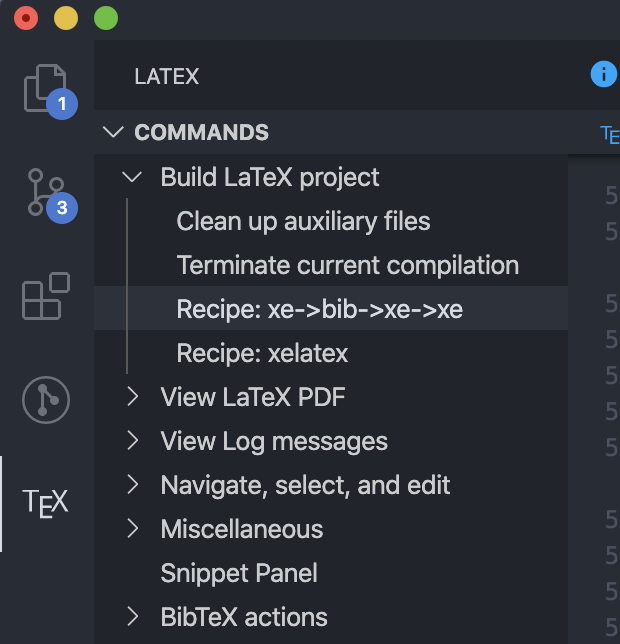
\includegraphics[width=0.4\textwidth]{figures/vscode_4.png}
    \caption{vscode配置以后:四步走}
    \label{fig_install_texlive}
\end{figure}




\section{常用的一些东西} % (fold)
\label{sec:常用的一些东西}

用到相关的直接到这里复制,然后修改就行

\subsection{国际三线表格} % (fold)
\label{sub:国际三线表格}

\begin{table}[H]
    \centering
    \caption{二硫化钼纳米管参数}
    \begin{tabular}{cccccc} % 控制表格的格式,可以是l,c,r
    \toprule
    参数& m & n & \tabincell{c}{太长了\\换行一下\\原子数}  & 内径 & 长度\\
    \midrule
    数值 & 15 & 15  & 2880 & 2.3014nm & 9.95nm \\
    \bottomrule
    \end{tabular}
    \label{tbl_mos2_nanotube}
\end{table}

这个注意,有多少列,后面就要有多少个c \footnote{否则会报错:Extra alignment tab has been changed to cr.有什么报错百度一下一般就找到了},这个c表示这一列居中(center),靠左的话:l,右:r;

那个label后面的名字自己取,但是不能有重复,是为了引用,比如这样,表格\ref{tbl_mos2_nanotube},方程、图片也是这样引用的,好处是,中间加一个表格导致这个表格的序号变了也没事,你不用再去修改其他地方的引用

\begin{lstlisting}[language = tex]
\begin{table}[H]
    \centering
    \caption{二硫化钼纳米管参数}
    \begin{tabular}{cccccc} % 控制表格的格式,可以是l,c,r
    \toprule
    参数& m & n & 原子数  & 内径 & 长度\\
    \midrule
    数值 & 15 & 15  & 2880 & 2.3014nm & 9.95nm \\
    \bottomrule
    \end{tabular}
    \label{tbl_mos2_nanotube_2}
\end{table}
\end{lstlisting}

\subsection{换页表格} % (fold)

我是真的没想到有的人表格居然这么长,竟然能有三页。。。。


\begin{longtable}{cccccc} % 控制表格的格式,可以是l,c,r
    \caption{二硫化钼纳米管参数}\label{tbl_mos2_nanotube}\\
    \toprule
    参数& m & n & 原子数 & 内径 & 长度\\
    \midrule
    数值 & 15 & 15  & 2880 & 2.3014nm & 9.95nm \\
    数值1 & 15 & 15  & 2880 & 2.3014nm & 9.95nm \\
    数值2 & 15 & 15  & 2880 & 2.3014nm & 9.95nm \\
    数值3 & 15 & 15  & 2880 & 2.3014nm & 9.95nm \\
    数值4 & 15 & 15  & 2880 & 2.3014nm & 9.95nm \\
    数值5 & 15 & 15  & 2880 & 2.3014nm & 9.95nm \\
    数值6 & 15 & 15  & 2880 & 2.3014nm & 9.95nm \\
    数值7 & 15 & 15  & 2880 & 2.3014nm & 9.95nm \\
    数值8 & 15 & 15  & 2880 & 2.3014nm & 9.95nm \\
    数值9 & 15 & 15  & 2880 & 2.3014nm & 9.95nm \\
    数值10 & 15 & 15  & 2880 & 2.3014nm & 9.95nm \\
    数值11 & 15 & 15  & 2880 & 2.3014nm & 9.95nm \\
    数值12 & 15 & 15  & 2880 & 2.3014nm & 9.95nm \\
    数值13 & 15 & 15  & 2880 & 2.3014nm & 9.95nm \\
    数值14 & 15 & 15  & 2880 & 2.3014nm & 9.95nm \\
    数值15 & 15 & 15  & 2880 & 2.3014nm & 9.95nm \\
    数值16 & 15 & 15  & 2880 & 2.3014nm & 9.95nm \\
    数值17 & 15 & 15  & 2880 & 2.3014nm & 9.95nm \\
    数值18 & 15 & 15  & 2880 & 2.3014nm & 9.95nm \\
    数值19 & 15 & 15  & 2880 & 2.3014nm & 9.95nm \\
    数值20 & 15 & 15  & 2880 & 2.3014nm & 9.95nm \\
    \bottomrule
\end{longtable}

    

% subsection 国际三线表格 (end)


\subsection{字体} % (fold)
\label{sub:字体}

\begin{table}[H]
    \centering
    \caption{字体}
    \begin{tabular}{ccccccc} % 控制表格的格式
    \toprule
    名称& 加粗 & 倾斜 & 宋体  & 仿宋 & 黑体 \\
    \midrule
    显示 & \textbf{兰朵儿} & \textit{兰朵儿}  & \songti{兰朵儿} & \fangsong{兰朵儿} & \heiti{兰朵儿}  \\
    显示 & \textbf{ldr} & \textit{ldr}  & \songti{ldr} & \fangsong{ldr} & \heiti{ldr}  \\
    \bottomrule
    \end{tabular}
    \label{tbl_font}
\end{table}
发现没,中文斜体没有效果的,你可以自定义,这个自己百度吧;中文加粗已经解决了该问题,注意这个文件第四行,开启伪加粗(2020.5.18),可以用bfserie或者textbf但是注意,win上bfserie效果好一些,mac上textbf好一些

关于英文新罗马字体的说明:
在windows上,引用mathptmx包,正文、公式中的英文就会变成新罗马(Times New Roman)字体,但是mac系统上,没有任何效果,还是默认的罗马字体(和Times New Roman很相似,QR两个单词区分明显),所以我在2.1.3以及之后的模板中加入了以下两个命令:

\begin{lstlisting}[language = tex]
\RequirePackage{mathptmx} %加入这条命令会导致花体,mathcal和mathscr完全相同,正常mathcal会花的轻一些。
\RequirePackage{fontspec} %这一条在windows可有可无,效果相同,但是mac上必须。
\end{lstlisting}

但是mathptmx会导致花体,mathcal和mathscr完全相同,正常mathcal会花的轻一些。


% subsection 常用的 (end)

\subsection{公式} % (fold)
\label{sub:公式}
所有的符号都要用美元符号包裹\$,需要用到某一个但是不知道,直接百度,基本上都有
\begin{table}[H]
    \centering
    \caption{公式}
    \begin{tabular}{cccccccccc} % 控制表格的格式
    \toprule
    名称& 分数 & 下角标 & 上角标  & 矢量 & 根号 & 希腊字母 & 点乘 & 叉乘 & 矢量\\
    \midrule
    显示 & $\frac{1}{2}$ & $O_2$  & $a^2$ & $\vec{AB}$ & $\sqrt[2]{3}$ & $\theta$ & $\cdot$ & $\times$& $\vec{a}$\\
   
    \bottomrule
    \end{tabular}
    \label{tbl_gs}
\end{table}

但是有时候我们只是正文中想用$MoS_2$,它竟然斜体,不想斜体,我写了个命令,这样用\eqrm{MoS_2},正的吧,常用的命令可以自定义

% subsection 公式 (end)

\subsection{左边大括号} % (fold)
\label{sub:左边大括号}

\begin{equation}
    \left\{
    \begin{array}{rcl}
        \vec{e_1} &= \frac{3a}{2} \vec{i} + \frac{\sqrt{3a}}{2} \vec{j} \\
        \vec{e_2} &= \frac{3a}{2} \vec{i} - \frac{\sqrt{3a}}{2} \vec{j}
    \end{array}
    \right.
    \label{e1e2}
\end{equation}

注意后面有个方程的编号,如果想取消,把上下的两个$equation$改成$equation*$

\begin{equation*}
    \left\{
    \begin{array}{rcl}
        \vec{e_1} &= \frac{3a}{2} \vec{i} + \frac{\sqrt{3a}}{2} \vec{j} \\
        \vec{e_2} &= \frac{3a}{2} \vec{i} - \frac{\sqrt{3a}}{2} \vec{j}
    \end{array}
    \right.
    \label{e1e2_2}
\end{equation*}

% subsection 左边大括号 (end)

\subsection{复杂公式} % (fold)
\label{sub:复杂公式}
不会输出的符号,请百度,啥都有

\begin{equation}
\hat{HQR}=\frac{\epsilon}{2}\hat{\sigma}_{z}-\frac{\Delta}{2}\hat{\sigma}_{x}+\sum_{k}\omega_{k}\hat{b}_{k}^{\dagger}\hat{b}_{k}+\sum_{k}\frac{g_{k}}{2}\hat{\sigma}_{z}(\hat{b}_{k}+\hat{b}_{k}^{\dagger})\label{eq:sbm}
\end{equation}

% subsection 复杂公式 (end)


\subsection{等号对齐站} % (fold)
\label{sub:等号对齐站}

主要是用这个aligned放在了方程的环境里,等号前面\&控制对齐,每一行后面双斜杠换行

\begin{equation}
    \begin{aligned}
        \vec{CH} & = m\cdot \vec{e_1} + n\cdot \vec{e_2} \\
        & = \frac{3(m+n)a}{2} \vec{i} + \frac{\sqrt{3}(m-n)a}{2} \vec{j} 
    \end{aligned}
    \label{ch}
\end{equation}

% subsection 等号对齐站 (end)

\subsection{矩阵乘法} % (fold)
\label{sub:矩阵乘法}

其实就是几个array组合

\begin{equation}
    \left[ 
    \begin{array}{c}
    x'\\
    y'\\
    \end{array}
    \right]=
    \left[ 
    \begin{array}{cc}
    cos \theta & sin \theta \\
    - sin \theta & cos \theta 
    \end{array}
    \right]
    \cdot
    \left[ 
    \begin{array}{c}
        x\\
        y\\
    \end{array}
    \right]
\end{equation}
% subsection 矩阵乘法 (end)


\subsection{图,并列排} % (fold)
\label{sub:图_并列排}

这一句代表这个图片宽度为一行文本宽度的$\frac{3}{10}$
\begin{lstlisting}[language = tex]
width=0.3\textwidth
\end{lstlisting}



\begin{figure}[H]
	\centering
	\subfloat[首页]{
        \includegraphics[width=0.3\textwidth]{figures/ldr1.jpg}
    }
	\subfloat[课表]{
        \includegraphics[width=0.3\textwidth]{figures/ldr2.jpg}
    }
	\subfloat[我的]{
        \includegraphics[width=0.3\textwidth]{figures/ldr4.jpg}
    }\\	
    \caption{i兰大易班截图}
    \label{fig_ldr}
\end{figure}

% subsection 图_并列排 (end)


\subsection{附页代码} % (fold)
\label{sub:附页代码}
可以在LZUThesis.clc里面修改代码格式

java代码
\begin{lstlisting}[language = java]
    System.out.print("i兰大易班")
    // 试一下中文注释
\end{lstlisting}


tex代码
\begin{lstlisting}[language = tex]
    width=0.3\textwidth
    % 注释
\end{lstlisting}

python代码
\begin{lstlisting}[language = python]
    print("i兰大易班")
    # 注释
\end{lstlisting}

matlab代码有专门的库,但是没必要高亮太多,而且中文适配有问题,直接按照下面这个就可以
\begin{lstlisting}[language = matlab]
    display("i兰大易班")
    % 注释
\end{lstlisting}

% subsection 附页代码 (end)

\subsection{参考文献} % (fold)
\label{sub:参考文献}

这个,百度学术、谷歌学术等网站都可以导出bibtex格式的参考文献(知网不行,网上有个人写了个转换器,但是windows用不了,就不放了,尽量用谷歌学术把那个文献找出来吧),直接放在bib/database.bib文件里、知网需要用其他东西转换,但是我建议用mendeley这个软件管理文献,然后可以导出bibtex格式的,甚至可以直接复制引用,很方便\cite{partl2016, tenne1992polyhedral, tussyadiah2015hotels}。

有些人希望多个参考文献同时引用时用[1-3]而不是[1,2,3],所以我加了个包cite。(2020-5-18)

具体怎么用可以百度,我这里告诉你什么可以用,但是具体的,建议百度,更靠谱一些。


有参考文献时,编译要经过4步,直接XeLaTeX --> BibTeX --> XeLaTeX --> XeLaTeX,不然很多问题,vscode配置以后很方便,以下内容放在设置中,重新打开vscode即可



% subsection 参考文献 (end)

% section 图标等常用的教程 (end)

\subsection{引用图、表、公式、章节} % (fold)

为什么要引用?不直接写数字?因为图表顺序变化时,引用的地方会自动变化。每次更加新引用,请四步走编译

引用的地方加label,自己写个名字,可以是中文,然后引用的地方如下:

如图\ref{fig_ldr}所示

如公式\eqref{e1e2}所示,会自动带括号

如表\ref{tbl_gs}所示

在\ref{sub:参考文献}中已经提及


%论文后部
\backmatter


%=======%
%引入参考文献文件
%=======%
\bibdatabase{bib/database}%bib文件名称 仅修改bib/ 后部分
\printbib
% \nocite{*} %显示数据库中有的,但是正文没有引用的文献



\Appendix


这里是附录页,附上你的程序或必要的相关知识

{\bfseries 编译方式:} XeLaTeX -->BibTeX --> XeLaTeX-->XeLaTeX


\Thanks

这里是致谢页,你可以在这里致谢你的舍友,老师,朋友,或者我。


%=====%
%论文(设计)成绩:注意2007的模板要求,成绩页在最后,2020要求成绩页在摘要前面
%=====%

% 下面这些注释掉可以去掉成绩、评语什么的
\supervisorcomment{导师评价你人很好}


\committeecomment{优秀}

\finalgrade{100}
% 上面这些注释掉可以去掉成绩、评语什么的

\Grade %这一句才是成绩页,上面是填写


\end{document}